
\documentclass[11pt]{article}
\usepackage{hyperref}
\usepackage{makecell}
\usepackage{blindtext}
\usepackage{xcolor}
\usepackage{enumitem}
\usepackage{listings}
\hypersetup{
    colorlinks=true,
    linkcolor=blue,
    filecolor=magenta,      
    urlcolor=red,
    pdftitle={Overleaf Example},
    pdfpagemode=FullScreen,
    }
\usepackage{amsmath,amssymb,amsfonts}
\usepackage{graphicx}

\setlength{\topmargin}{-.5in} \setlength{\textheight}{9.25in}
\setlength{\oddsidemargin}{0in} \setlength{\textwidth}{6.8in}

%%%%%%%%%%%%%%%%%%%%%%%%%%%%%%%%%%%%%%%%%%
\usepackage{pythonhighlight}
%%%%%%%%%%%%%%%%%%%%%%%%%%%
\newcounter{mycounter} % create a new counter, called 'mycounter'
% default def'n of '\themycounter' is '\arabic{mycounter}'
%% command to increment 'mycounter' by 1 and to display its value:
\newcommand\showmycounter{\stepcounter{mycounter}\themycounter}
\usepackage{lipsum}
\newcommand\showlips{\stepcounter{mycounter}\lipsum[\value{mycounter}]}
%%%%%%%%%%%%%%%%%%%%%%%%%%%%%%%%%%%%%%
\usepackage{framed}
\usepackage{hyperref}
\usepackage{fancyhdr}

%%%%%%%%%%%%%%%%%%%%%%%%%%%%%%%%%%%%%%%%%%%%%%%%%%%%%%%%%%%%%
\usepackage{listings}
\usepackage{xcolor}

\definecolor{codegreen}{rgb}{0,0.6,0}
\definecolor{codegray}{rgb}{0.5,0.5,0.5}
\definecolor{codepurple}{rgb}{0.58,0,0.82}
\definecolor{backcolour}{rgb}{0.95,0.95,0.92}

\lstdefinestyle{mystyle}{
    backgroundcolor=\color{backcolour},   
    commentstyle=\color{codegreen},
    keywordstyle=\color{magenta},
    numberstyle=\tiny\color{codegray},
    stringstyle=\color{codepurple},
    basicstyle=\ttfamily\footnotesize,
    breakatwhitespace=false,         
    breaklines=true,                 
    captionpos=b,                    
    keepspaces=true,                 
    numbers=left,                    
    numbersep=5pt,                  
    showspaces=false,                
    showstringspaces=false,
    showtabs=false,                  
    tabsize=2
}

\lstset{style=mystyle}
%%%%%%%%%%%%%%%%%%%%%%%%%%%%%%%%%%%%%%%%%%%%%%%%%%%%%%%%%%%%%
\title{\LARGE AI VIET NAM – RESEARCH TEAM}
\author{\Large SELF-ATTENTION GENERATIVE ADVERSARIAL NETWORKS}
\pagestyle{fancy}
\fancyhf{}
\lhead{\bfseries AI VIETNAM}
\rhead{\bfseries  aivietnam.edu.vn}
\begin{document}
\maketitle
%\Largebf Ma 12 Long Test 1\hfill 9 February 2017}
%\medskip\hr
%\noindent{\ule

\begin{enumerate}[\arabic*]
    \item
    \textbf{Purpose/outputs:}
    \begin{itemize}
        \item \textbf{Self-Attention Generative Adversarial Network (SAGAN)} \cite{https://doi.org/10.48550/arxiv.1805.08318} allows attention-driven, long-range dependency modeling for image generation tasks. 
        \item Details in SAGAN may be created utilizing cues from all feature locations. Furthermore, the discriminator can ensure that highly detailed elements in different parts of the image are consistent with one another.
        \item The proposed SAGAN significantly outperforms prior work in image synthesis by boosting the best reported Inception score from 36.8 to 52.52 and reducing Fréchet Inception distance from 27.62 to 18.65 \cite{https://doi.org/10.48550/arxiv.1706.08500} on the challenging ImageNet dataset \cite{5206848}.
    \end{itemize}
        
    \item
    \textbf{Methodology:}
    \begin{itemize}
        \item \textbf{The self-attention module} is complementary to convolutions and helps with modeling long range, multi-level dependencies across image regions. Armed with self-attention, the generator can draw images in which fine details at every location are carefully coordinated with fine details in distant portions of the image. Applying self-attention to the GAN framework (see \hyperref[fig:self attention]{Figure 1}) enables both the generator and the discriminator to efficiently model relationships between widely separated spatial regions. \\
        \begin{figure}
            \centering
            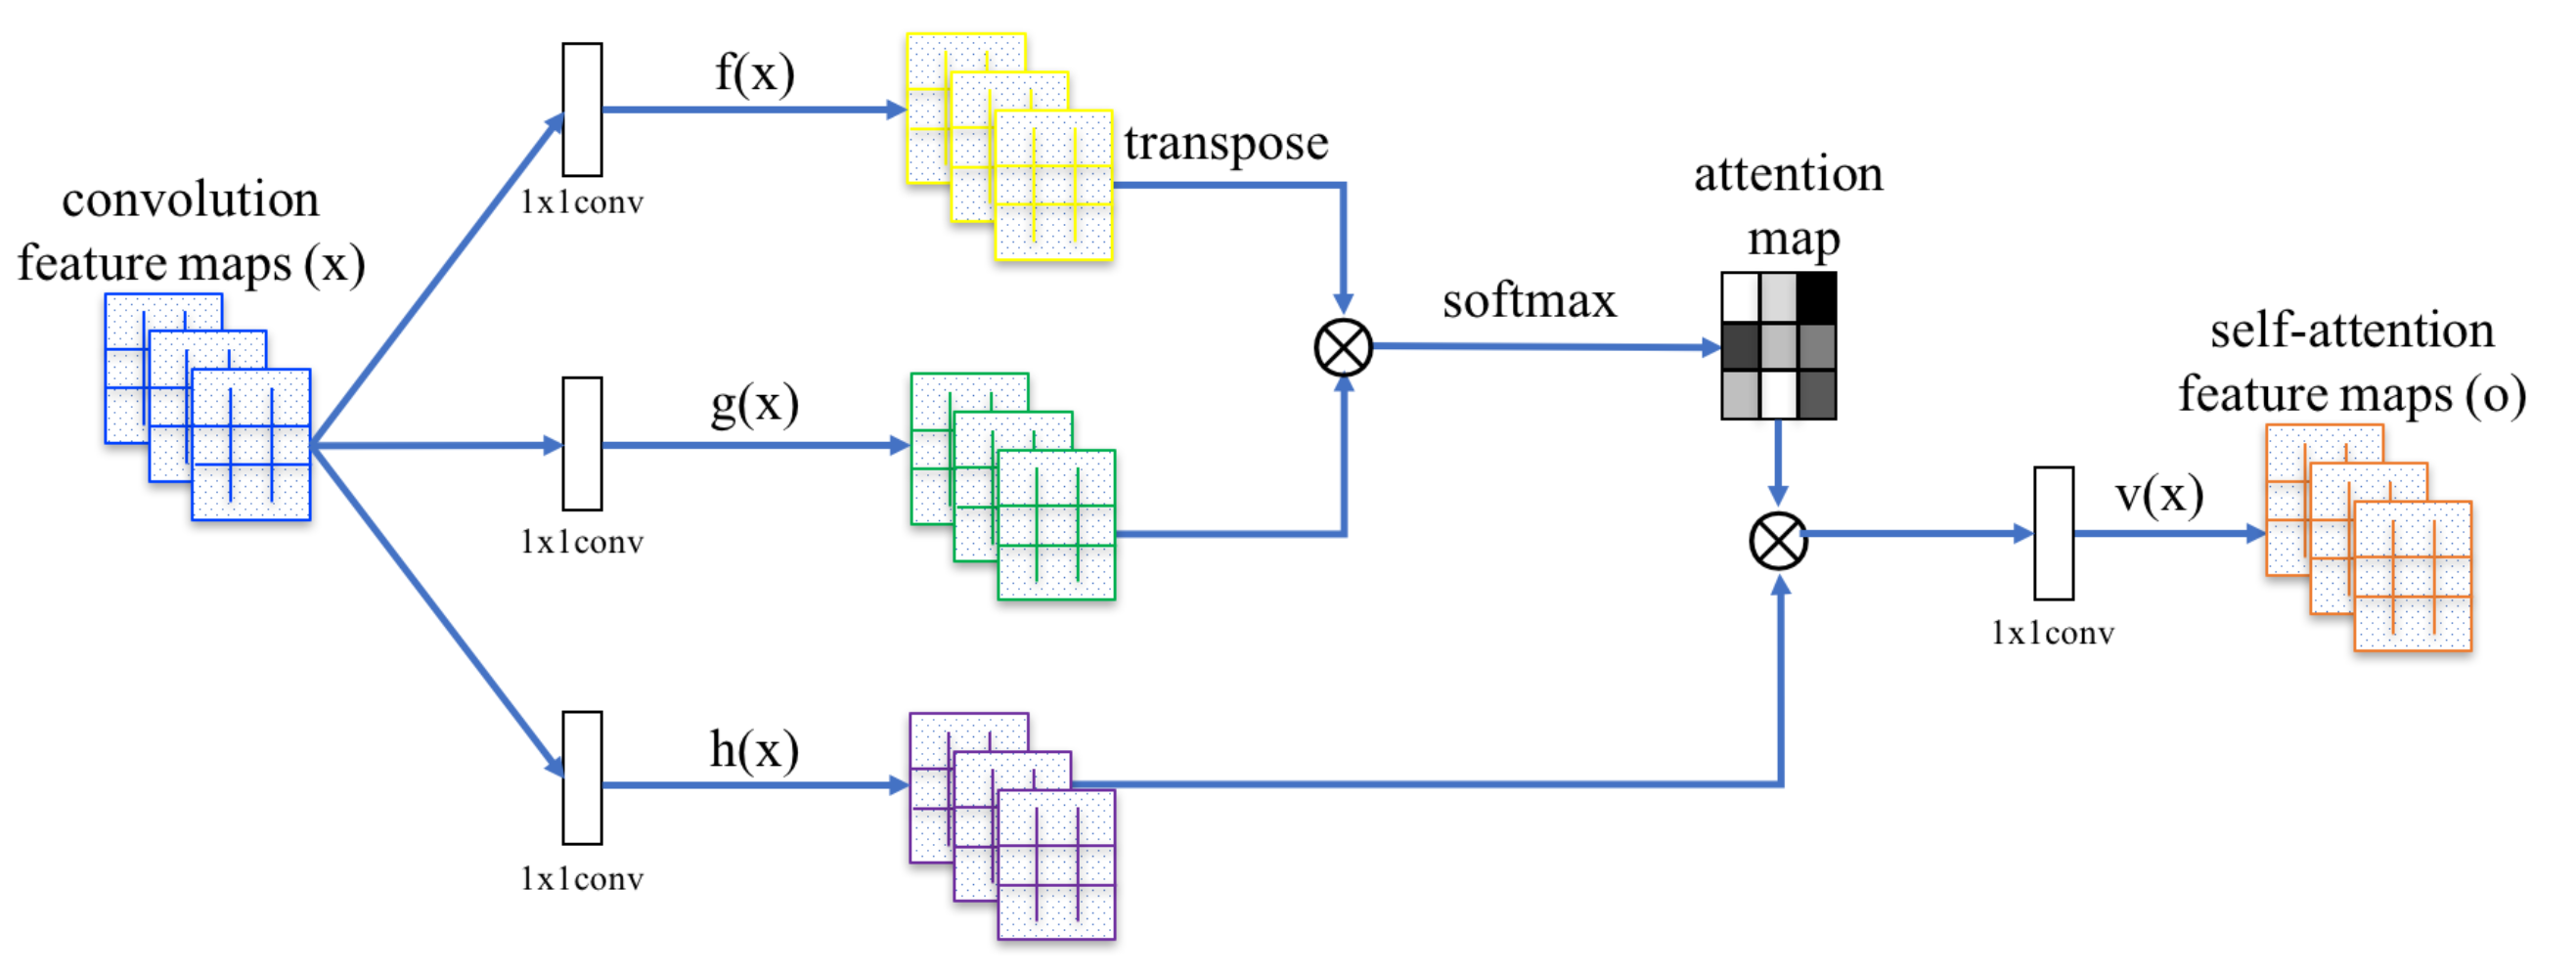
\includegraphics[width=15cm]{self attention module.png}
            \caption{The proposed self-attention module for the SAGAN. The softmax operation is performed on each row.}
            \label{fig:self attention}
        \end{figure}
        
The image features from the previous hidden layer $\boldsymbol{x} \in$ $\mathbb{R}^{C \times N}$ are first transformed into two feature spaces $\boldsymbol{f}, \boldsymbol{g}$ to calculate the attention, where $f(x)=W_f x, g(x)=$ $W_g \boldsymbol{x}$.\\

Here, $C$ is the number of channels and $N$ is the number of feature locations of features from the previous hidden layer. $\beta_{j, i}$ indicates the extent to which the model attends to the $i^{\text {th }}$ location when synthesizing the $j^{t h}$ region and could be written as:
$$
\beta_{j, i}=\frac{\exp \left(s_{i j}\right)}{\sum_{i=1}^N \exp \left(s_{i j}\right)},
$$
where $s_{i j}=\boldsymbol{f}\left(\boldsymbol{x}_{\boldsymbol{i}}\right)^T \boldsymbol{g}\left(\boldsymbol{x}_{\boldsymbol{j}}\right)$ \\

The output of the attention layer is $\boldsymbol{o}=\left(\boldsymbol{o}_1, \boldsymbol{o}_2, \ldots, \boldsymbol{o}_j, \ldots, \boldsymbol{o}_N\right) \in$ $\mathbb{R}^{C \times N}$, where,
$$
\boldsymbol{o}_{\boldsymbol{j}}=\boldsymbol{v}\left(\sum_{i=1}^N \beta_{j, i} \boldsymbol{h}\left(\boldsymbol{x}_{\boldsymbol{i}}\right)\right), \boldsymbol{h}\left(\boldsymbol{x}_{\boldsymbol{i}}\right)=\boldsymbol{W}_{\boldsymbol{h}} \boldsymbol{x}_{\boldsymbol{i}}, \boldsymbol{v}\left(\boldsymbol{x}_{\boldsymbol{i}}\right)=\boldsymbol{W}_{\boldsymbol{v}} \boldsymbol{x}_{\boldsymbol{i}} .
$$
In the above formulation, $\boldsymbol{W}_{\boldsymbol{g}} \in \mathbb{R}^{\bar{C} \times C}, \boldsymbol{W}_{\boldsymbol{f}} \in \mathbb{R}^{\bar{C} \times C}$, $\boldsymbol{W}_{\boldsymbol{h}} \in \mathbb{R}^{\bar{C} \times C}$, and $\boldsymbol{W}_{\boldsymbol{v}} \in \mathbb{R}^{C \times \bar{C}}$ are the learned weight matrices, which are implemented as $1 \times 1$ convolutions.

In addition, the output of the attention layer is scaled by a parameter and add back the input feature map. Therefore, the final output is given by,
$$
\boldsymbol{y}_i=\gamma \boldsymbol{o}_i+\boldsymbol{x}_{\boldsymbol{i}},
$$
where $\gamma$ is a learnable scalar and it is initialized as 0 . Introducing the learnable $\gamma$ allows the network to first rely on the cues in the local neighborhood – since this is easier – and then gradually learn to assign more weight to the non-local evidence. \\

\item See \hyperref[fig:attention visualization]{Figure 2} for visualization of attention maps. It can be observed that the network learns to allocate attention according to similarity of color and texture, rather than just spatial adjacency. In addition to that, while some query points are quite close in spatial location, their attention maps can be very different.\\

\begin{figure}[!ht]
    \centering
    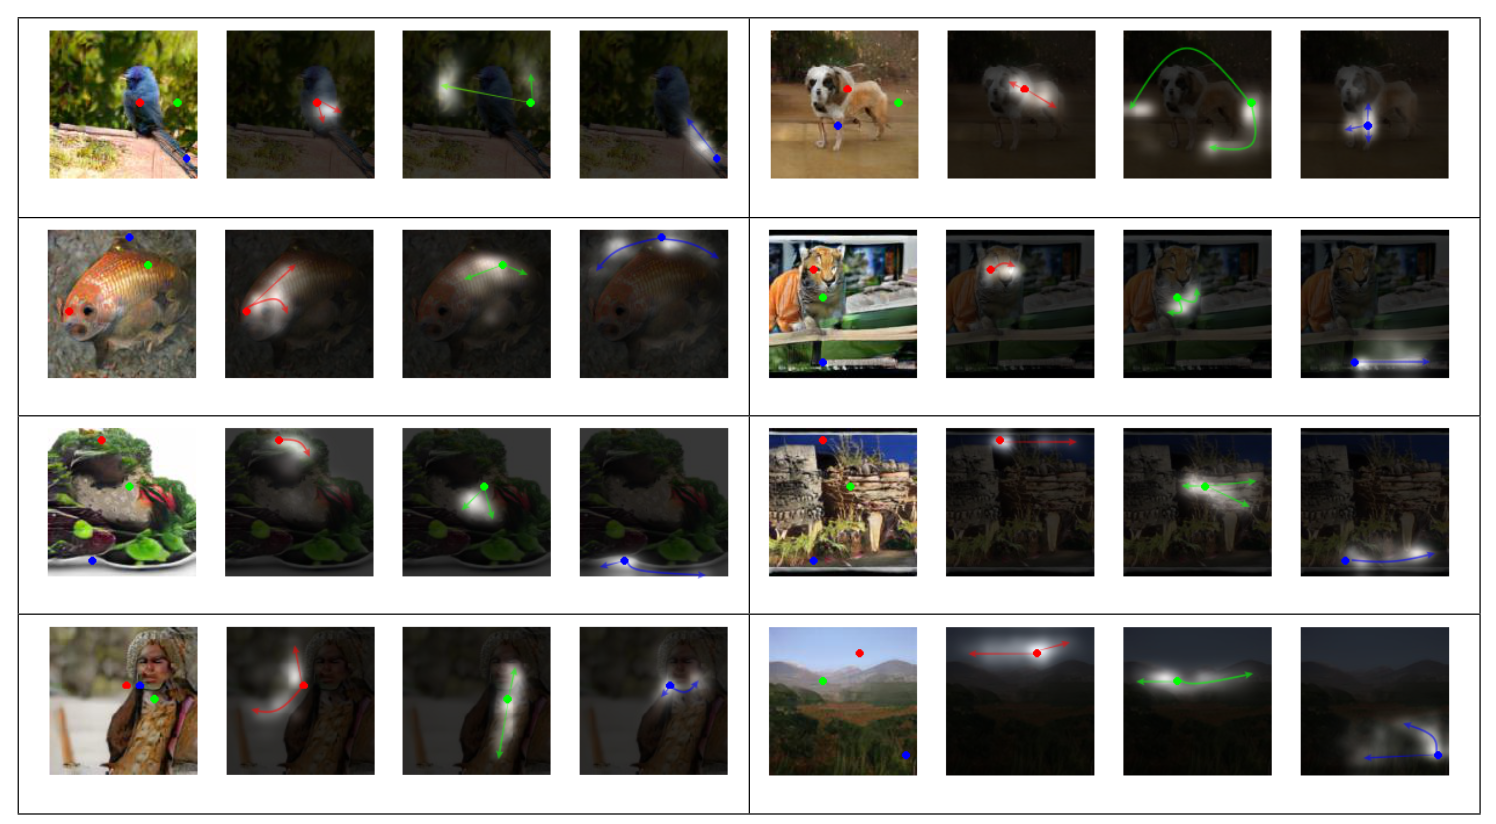
\includegraphics[width=16cm]{attention visualization.png}
    \caption{Visualization of attention maps of the last generator layer that used attention. These images were generated by SAGAN. The network learns to allocate attention according to similarity of color and texture, rather than just spatial adjacency.}
    \label{fig:attention visualization}
\end{figure}

        \item GAN generators using the \textbf{spectral normalization technique} that has previously been applied only to the discriminator \cite{https://doi.org/10.48550/arxiv.1802.05957}.\\
        
         \item Spectral normalization does not require extra hyper-parameter tuning (setting the spectral norm of all weight layers to 1 consistently performs well in practice). Moreover, the computational cost is also relatively small.\\

         \item Applying spectral normalization of both generator and discriminator makes it possible to use fewer discriminator updates per generator update, thus significantly reducing the computational cost of training. The approach also shows more stable training behavior.

    \end{itemize}
    
    \item
    \textbf{Results:}   
    \begin{itemize}
        \item SAGAN achieves much better performance (i.e., lower intra FID) than the state-of-the-art GAN model for synthesizing image classes with complex geometric or structural patterns (see \hyperref[fig:result]{Figure 3}).
        \item  The self-attention in SAGAN is complementary to the convolution for capturing long-range, global-level depen- dencies occurring consistently in geometric or structural patterns, but plays a similar role as the local convolution when modeling dependencies for simple texture.
        \begin{figure}[!ht]
        \centering
        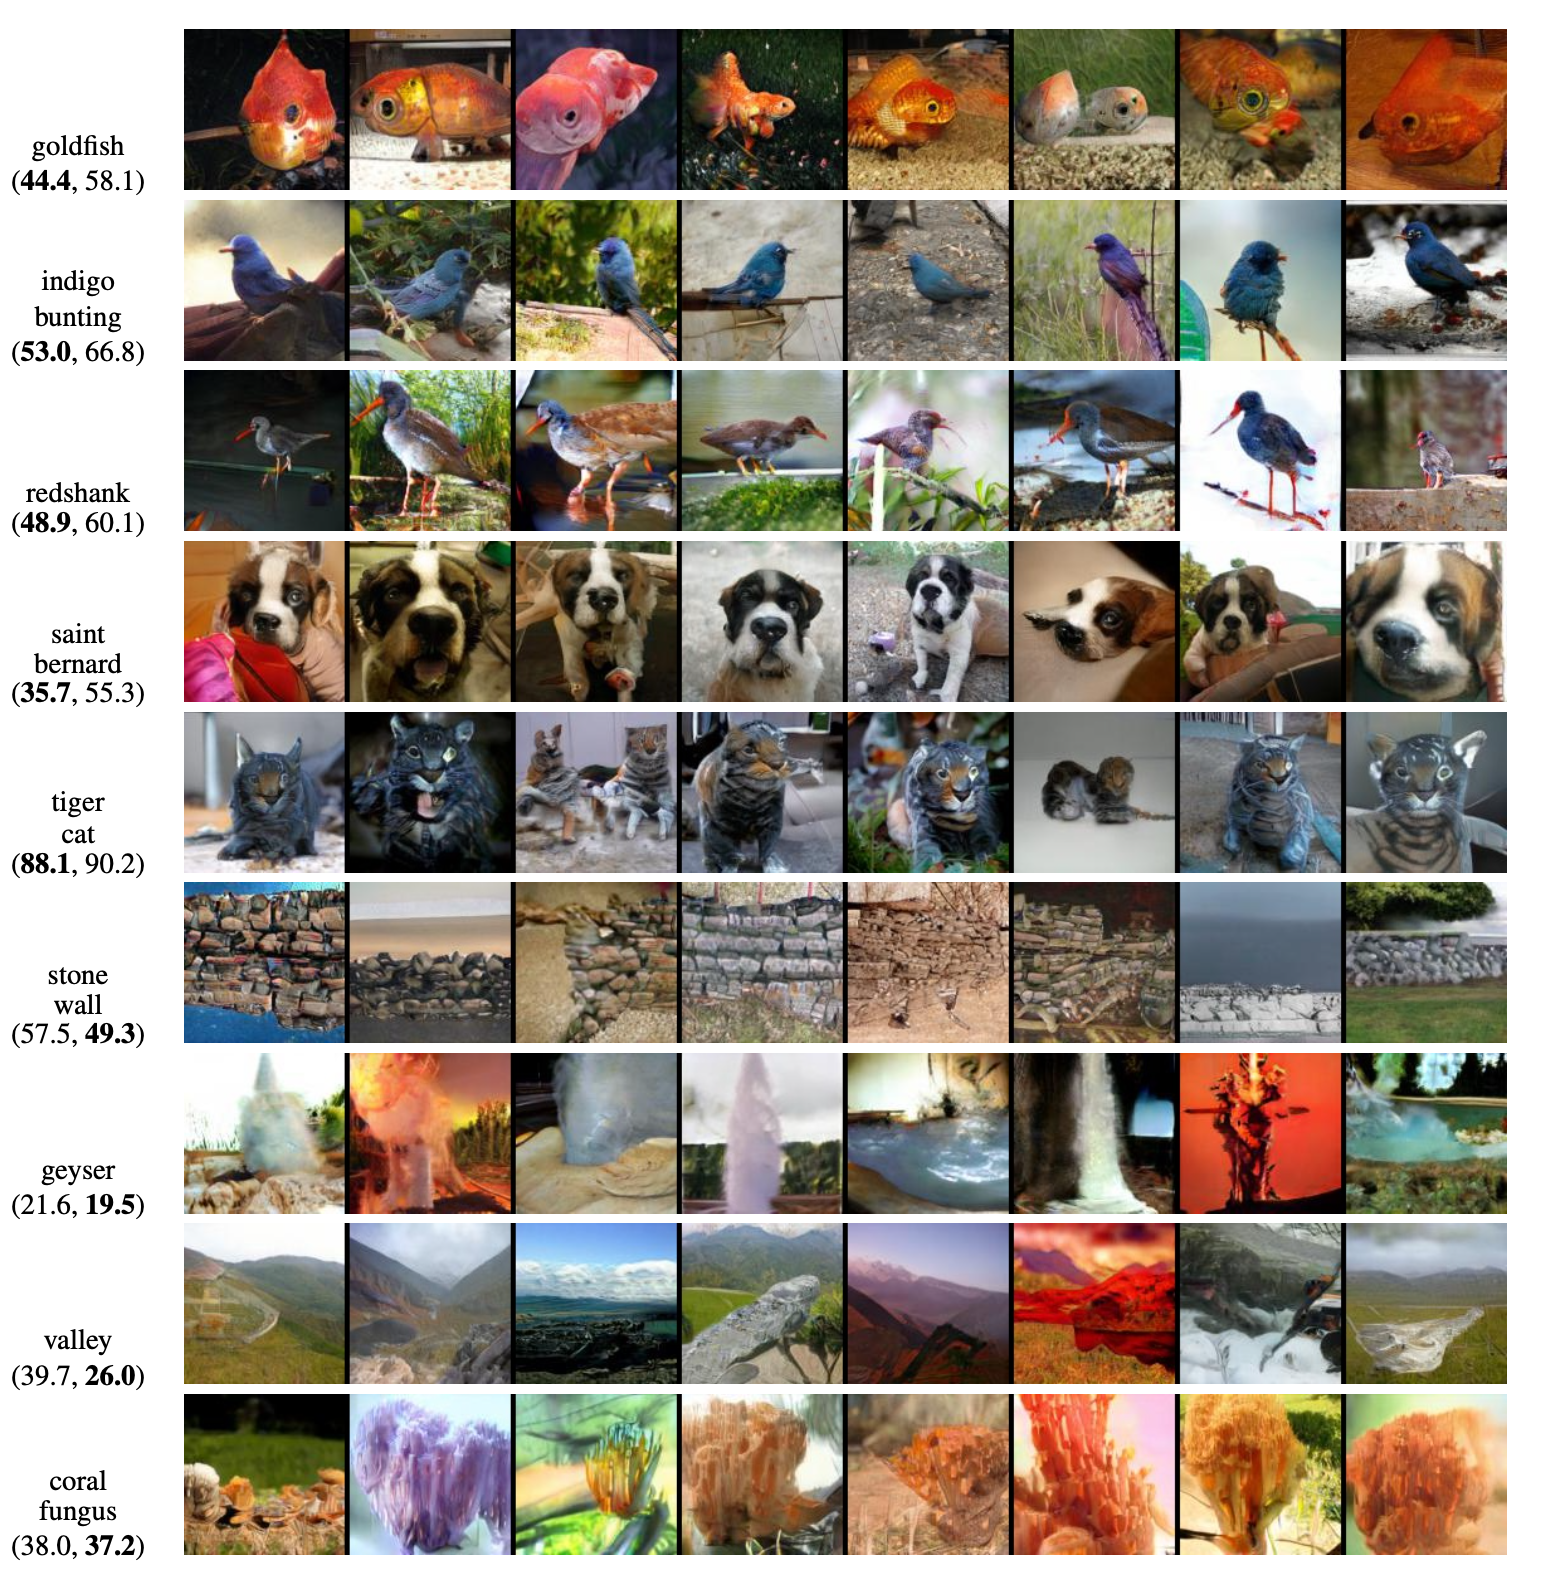
\includegraphics[width=17cm]{result.png}
        \caption{$128 \times 128$ example images generated by SAGAN for different classes.}
        \label{fig:result}
    \end{figure}
    \end{itemize}
    
\end{enumerate}
\nocite{*}
\pagebreak

\bibliographystyle{abbrv}
\bibliography{citation}
\end{document} 